\RequirePackage{currfile}
\documentclass[12pt]{beamer}
\usepackage[utf8]{inputenc}
\usepackage[spanish]{babel}
\usepackage{standalone}
\usepackage{color}
\usepackage{siunitx}
\usepackage{hyperref}
%\hypersetup{colorlinks,linkcolor=,urlcolor=blue}
%\hypersetup{colorlinks,urlcolor=blue}
\usepackage{xcolor,soul}
\usepackage{etoolbox}
\usepackage{amsmath}
\usepackage{amsthm}
\usepackage{physics}
\usepackage{multicol}
\usepackage{bookmark}
\usepackage{longtable}
\usepackage{listings}
\usepackage{graphicx}
\usepackage{tikz}
\usepackage[siunitx, RPvoltages]{circuitikz}
\usetikzlibrary{arrows, patterns, matrix, backgrounds, decorations, shapes, decorations.markings, decorations.pathmorphing}
\usepackage[autostyle,spanish=mexican]{csquotes}
\usepackage[os=win]{menukeys}
\usepackage{pifont}
\usepackage{pbox}
\usepackage{caption}
\captionsetup{font=scriptsize,labelfont=scriptsize}
%\usepackage[sfdefault]{roboto}  %% Option 'sfdefault' only if the base font of the document is to be sans serif

%Sección de definición de colores
\definecolor{ao}{rgb}{0.0, 0.5, 0.0}
\definecolor{bisque}{rgb}{1.0, 0.89, 0.77}
\definecolor{amber}{rgb}{1.0, 0.75, 0.0}
\definecolor{armygreen}{rgb}{0.29, 0.33, 0.13}
\definecolor{alizarin}{rgb}{0.82, 0.1, 0.26}
\definecolor{cadetblue}{rgb}{0.37, 0.62, 0.63}
\definecolor{deepblue}{rgb}{0,0,0.5}
\definecolor{brown}{rgb}{0.59, 0.29, 0.0}
\definecolor{OliveGreen}{rgb}{0,0.25,0}


\usefonttheme[onlymath]{serif}
%Sección de definición de nuevos comandos

\newcommand*{\TitleParbox}[1]{\parbox[c]{1.75cm}{\raggedright #1}}%
\newcommand{\python}{\texttt{python}}
\newcommand{\textoazul}[1]{\textcolor{blue}{#1}}
\newcommand{\azulfuerte}[1]{\textcolor{blue}{\textbf{#1}}}
\newcommand{\funcionazul}[1]{\textcolor{blue}{\textbf{\texttt{#1}}}}
\newcommand{\ptilde}[1]{\ensuremath{{#1}^{\prime}}}
\newcommand{\ptildosargs}[2]{\ensuremath{{#1}^{\prime \, ({#2})}}}
\newcommand{\stilde}[1]{\ensuremath{{#1}^{\prime \prime}}}
\newcommand{\ttilde}[1]{\ensuremath{{#1}^{\prime \prime \prime}}}
\newcommand{\ntilde}[2]{\ensuremath{{#1}^{(#2)}}}
\renewcommand{\arraystretch}{1.5}

\newcounter{saveenumi}
\newcommand{\seti}{\setcounter{saveenumi}{\value{enumi}}}
\newcommand{\conti}{\setcounter{enumi}{\value{saveenumi}}}
\renewcommand{\rmdefault}{cmr}% cmr = Computer Modern Roman

\linespread{1.5}

\usefonttheme{professionalfonts}
%\usefonttheme{serif}
\DeclareGraphicsExtensions{.pdf,.png,.jpg}


%Sección para el tema de beamer, con el theme, usercolortheme y sección de footers
\mode<presentation>
{
  \usetheme{CambridgeUS}
  \setbeamertemplate{headline}{}
  %\useoutertheme{infolines}
  \useoutertheme{default}
  \usecolortheme{rose}
  \setbeamercovered{invisible}
  % or whatever (possibly just delete it)
  \setbeamertemplate{section in toc}[sections numbered]
  \setbeamertemplate{subsection in toc}[subsections numbered]
  \setbeamertemplate{subsection in toc}{\leavevmode\leftskip=3.2em\rlap{\hskip-2em\inserttocsectionnumber.\inserttocsubsectionnumber}\inserttocsubsection\par}
  \setbeamercolor{section in toc}{fg=blue}
  \setbeamercolor{subsection in toc}{fg=blue}
  \setbeamercolor{frametitle}{fg=blue}

  \setbeamertemplate{footline}
  %\beamertemplatenavigationsymbolsempty
}

\makeatletter
\setbeamercolor{section in foot}{bg=gray!30, fg=black!90!orange}
\setbeamercolor{subsection in foot}{bg=blue!30!yellow, fg=red}
\setbeamertemplate{footline}
{
  \leavevmode%
  \hbox{%
  \begin{beamercolorbox}[wd=.333333\paperwidth,ht=2.25ex,dp=1ex,center]{section in foot}%
    \usebeamerfont{section in foot} \insertsection
  \end{beamercolorbox}}%
  \begin{beamercolorbox}[wd=.333333\paperwidth,ht=2.25ex,dp=1ex,center]{subsection in foot}%
    \usebeamerfont{subsection in foot}  \insertsubsection
  \end{beamercolorbox}%
  \begin{beamercolorbox}[wd=.333333\paperwidth,ht=2.25ex,dp=1ex,right]{date in head/foot}%
    \usebeamerfont{date in head/foot} \insertshortdate{} \hspace*{2em}
    \insertframenumber{} / \inserttotalframenumber \hspace*{2ex} 
  \end{beamercolorbox}}%
  \vskip0pt%
\makeatother  

\makeatletter
\patchcmd{\beamer@sectionintoc}
  {\vfill}
  {\vskip\itemsep}
  {}
  {}
\makeatother

% \makeatletter
% \patchcmd{\hyper@link@}
%   {{\Hy@tempb}{#4}}
%   {{\Hy@tempb}{\ul{#4}}}
%   {}{}
% \makeatother


% Sección para el código

\definecolor{Code}{rgb}{0,0,0}
\definecolor{Keywords}{rgb}{255,0,0}
\definecolor{Strings}{rgb}{255,0,255}
\definecolor{Comments}{rgb}{0,0,255}
\definecolor{Numbers}{rgb}{255,128,0}

\DeclareCaptionFont{white}{\color{white}}
\DeclareCaptionFormat{listing}{\colorbox{gray}{\parbox{0.99\textwidth}{#1#2#3}}}
\captionsetup[lstlisting]{format=listing,labelfont=white,textfont=white}
\renewcommand{\lstlistingname}{Código}

\lstset{
basicstyle=\ttfamily,
columns=fullflexible,
breaklines=true
}

\lstdefinestyle{codigopython}{%
  language=Python,                % choose the language of the code
  %basicstyle=\footnotesize\small,       % the size of the fonts that are used for the code
  numbers=left,                   % where to put the line-numbers
  numberstyle=\scriptsize,      % the size of the fonts that are used for the line-numbers
  stepnumber=1,                   % the step between two line-numbers. If it is 1 each line will be numbered
  numbersep=5pt,                  % how far the line-numbers are from the code
  backgroundcolor=\color{white},  % choose the background color. You must add \usepackage{color}
  showspaces=false,               % show spaces adding particular underscores
  showstringspaces=false,         % underline spaces within strings
  showtabs=false,                 % show tabs within strings adding particular underscores
  frame=single,   		% adds a frame around the code
  tabsize=2,  		% sets default tabsize to 2 spaces
  captionpos=t,   		% sets the caption-position to bottom
  breaklines=true,    	% sets automatic line breaking
  breakatwhitespace=false,    % sets if automatic breaks should only happen at whitespace
  escapeinside={\#},  % if you want to add a comment within your code
  stringstyle =\color{OliveGreen},
  texcl = true,
  %otherkeywords={{as}},             % Add keywords here
  keywordstyle = \color{blue},
  commentstyle = \color{black},
  identifierstyle = \color{black},
  % literate=%
  %         {á}{{\'a}}1
  %         {é}{{\'e}}1
  %         {í}{{\'i}}1
  %         {ó}{{\'o}}1
  %         {ú}{{\'u}}1
  %
  %keywordstyle=\ttb\color{deepblue}
  %fancyvrb = true,
literate={0}{{\textcolor{red}{0}}}{1}%
            {1}{{\textcolor{red}{1}}}{1}%
            {2}{{\textcolor{red}{2}}}{1}%
            {3}{{\textcolor{red}{3}}}{1}%
            {4}{{\textcolor{red}{4}}}{1}%
            {5}{{\textcolor{red}{5}}}{1}%
            {6}{{\textcolor{red}{6}}}{1}%
            {7}{{\textcolor{red}{7}}}{1}%
            {8}{{\textcolor{red}{8}}}{1}%
            {9}{{\textcolor{red}{9}}}{1}%
            {.0}{{\textcolor{red}{.0}}}{2}% Following is to ensure that only periods
            {.1}{{\textcolor{red}{.1}}}{2}% followed by a digit are changed.
            {.2}{{\textcolor{red}{.2}}}{2}%
            {.3}{{\textcolor{red}{.3}}}{2}%
            {.4}{{\textcolor{red}{.4}}}{2}%
            {.5}{{\textcolor{red}{.5}}}{2}%
            {.6}{{\textcolor{red}{.6}}}{2}%
            {.7}{{\textcolor{red}{.7}}}{2}%
            {.8}{{\textcolor{red}{.8}}}{2}%
            {.9}{{\textcolor{red}{.9}}}{2}%
            {\ }{{ }}{1}% handle the space
        ,%
        %mathescape=true
        %escapeinside={*@}
        escapeinside={A_}{_B}
}

\title{Tema 3 - Ecuaciones diferenciales ordinarias}
\subtitle{Curso de Física Computacional}
\author[]{M. en C. Gustavo Contreras Mayén}
\begin{document}
\maketitle
\fontsize{14}{14}\selectfont
\spanishdecimal{.}
\section*{Contenido}
\frame{\tableofcontents[currentsection, hideallsubsections]}
\section{Introducción}
\frame{\tableofcontents[currentsection, hideothersubsections]}
\subsection{Motivación}
\begin{frame}
\frametitle{Introducción}
La importancia particular de los métodos numéricos para resolver ecuaciones diferenciales ordinarias (EDO) o sus sistemas se debe al hecho de que muchas de las leyes de la naturaleza se expresan convenientemente en forma diferencial.
\end{frame}
\begin{frame}
\frametitle{Introducción}
Las ecuaciones clásicas de movimiento de partículas, las ecuaciones de difusión de masa o transporte de calor, o la ecuación de onda de Schrödinger son solo algunos ejemplos que ilustran la extraordinaria diversidad de fenómenos físicos esencialmente diferentes, que se modelan mediante ecuaciones diferenciales.
\end{frame}
\begin{frame}
\frametitle{Introducción}
Una multitud de fenómenos se describen mediante ecuaciones diferenciales parciales (EDP), lo que implica derivadas de varios órdenes de la función desconocida con respecto a varias variables independientes.
\end{frame}
\begin{frame}
\frametitle{Introducción}
Nuevamente, en muchas situaciones, uno tiene que lidiar con las EDO dependiendo de las derivadas de varios órdenes de la función desconocida con respecto a una sola variable independiente.
\end{frame}
\begin{frame}
\frametitle{Introducción}
Las EDO pueden ser intrínsecamente ordinarias, es decir, pueden resultar como tales del modelado mismo del fenómeno en cuestión, o pueden resultar de un proceso previo de separación de variables de una EDP inicial, generalmente aprovechando ciertas propiedades de simetría presentadas por el sistema modelado.
\end{frame}
\begin{frame}
\frametitle{Introducción}
En una situación más compleja, la solución puede comprender varias funciones desconocidas, que satisfacen un sistema de EDO acopladas.
\end{frame}
\begin{frame}
\frametitle{Conexión en una EDO y un sistema de EDO}
Como ejemplo que muestra la conexión cerca entre EDO de orden superior y sistemas de EDO, consideremos el ejemplo clásico de la primera ley de Newton, que expresa la ecuación de movimiento de una partícula de masa $m$, experimentando una fuerza $F(x)$:
\begin{align}
m \, \dv[2]{x}{t} =  F(x)
\label{eq:ecuacion_12_01}
\end{align}
\end{frame}
\begin{frame}
\frametitle{Ejemplo de la mecánica}
Definiendo el momento de la partícula como $p = m \, (\dv*{x}{t})$, que es una EDO2 que puede descomponerse en un conjunto de dos ecuaciones diferenciales de primer orden:
\begin{align}
\dv{x}{t} = \dfrac{p}{m}, \hspace{0.5cm} \dv{p}{t} = F(x)
\label{eq:ecuacion_12_02}
\end{align}
que son las llamadas \emph{ecuaciones canónicas de Hamilton del movimiento}.
\end{frame}
\begin{frame}
\frametitle{Ejemplo de la mecánica}
Enfatizando en la velocidad de la partícula $v=p/m$ que su momento, las ecuaciones anteriores se vuelven
\begin{align}
\dv{x}{t} = v \hspace{0.5cm} \dv{v}{t} = \dfrac{1}{m} \, F(x)
\label{eq:ecuacion_12_03}
\end{align}
\end{frame}
\begin{frame}
\frametitle{Ejemplo de la mecánica}
Mediante la forma funcional equivalente de las EDO1 que componen este sistema acoplado, las dos funciones desconocidas, $x$ y $v$, se establecen en igualdad de condiciones.
\end{frame}
\begin{frame}
\frametitle{Ejemplo de la mecánica}
Además, la metodología de transformar la ecuación de movimiento inicial (\ref{eq:ecuacion_12_01}) en un sistema (\ref{eq:ecuacion_12_03}) revela que, en principio, es suficiente desarrollar solo métodos para resolver EDO1 o sistemas de tales ecuaciones.
\end{frame}
\begin{frame}
\frametitle{Alcance del Tema 3}
Sin embargo, debido a la importancia práctica particular de las ecuaciones de movimiento de segundo orden (por ejemplo en la dinámica molecular cuántica o clásica), se desarrollarán métodos numéricos específicos para resolver EDO o sistemas de segundo orden.
\end{frame}
\section{Ecuaciones Diferenciales Ordinarias}
\frame{\tableofcontents[currentsection, hideothersubsections]}
\subsection{Notación para las EDO}
\begin{frame}
\frametitle{Notación para las EDO}
Consideremos una ecuacion diferencial de orden $n$ (EDOn) para la función desconocida $y(t)$:
\begin{align}
\ntilde{y}{n} = f(t, y, \ptilde{y}, \ldots, \ntilde{y}{n-1})
\label{eq:ecuacion_12_04}
\end{align}
\end{frame}
\begin{frame}
\frametitle{Reducción de orden de la EDO}
Se puede demostrar fácilmente que la ecuación anterior, es equivalente a un sistema de $n$ EDO1:
\begin{align}
\ptilde{y}_{i} (t) = f_{i} (y, y_{1} (t), y_{2} (t), \ldots, y_{n} (t) ) \hspace{0.5cm} i = 1, 2, \ldots, n
\label{eq:ecuacion_12_05}
\end{align}
\end{frame}
\begin{frame}
\frametitle{Reducción de orden de las EDO}
Al considerar como funciones desconocidas además de $y$, también sus primeras $(n-1)$ derivadas
\begin{align*}
y_{i} \equiv \ntilde{y}{i-1}, \hspace{0.5cm} i = 1, 2, \ldots, n
\end{align*}
identificando la incógnita original con la primera de las nuevas funciones desconocidas, $y \equiv y_{1}$
\end{frame}
\begin{frame}
\frametitle{Nuevo sistema de ecuaciones}
Entonces el sistema que se obtiene, es de la forma:
\begin{align*}
\begin{cases}
\ptilde{y}_{i} (t) = y_{i+1} (t), \hspace{1cm} i = 1, 2, \ldots, n-1 \\
\ptilde{y}_{n} (t) = f(t, y_{1} (t), y_{2} (t), \ldots, y_{n} (t))
\end{cases}
\end{align*}
\end{frame}
\begin{frame}
\frametitle{Nuevo sistema de ecuaciones}
Donde las primeras $(n - 1$ ecuaciones resultan de notaciones simples y no son específicas, mientras que solo la última ecuación contiene la función particular del lado derecho $f$, que es específica del problema.
\end{frame}
\subsection*{Notación simplificada}
\begin{frame}
\frametitle{Notación simplificada}
Para simplificar la notación para el desarrollo de los métodos de solución numérica, el sistema general de EDO1 (ec. \ref{eq:ecuacion_12_05}), se puede escribir con una notación vectorial:
\begin{align}
\ptilde{y} (t) = f (t, y)
\label{eq:ecuacion_12_06}
\end{align}
\end{frame}
\begin{frame}
\frametitle{Notación simplificada}
Donde
\begin{align*}
y = \begin{bmatrix}
y_{1} (t) \\
\vdots \\
y_{n} (t)
\end{bmatrix}
\hspace{1.5cm}
f(t, y) =
\begin{bmatrix}
f_{1} (t, y_{1} (t), \ldots, y_{n} (t)) \\
\vdots \\
f_{n} (t, y_{1} (t), \ldots, y_{n} (t))
\end{bmatrix}
\end{align*}
\end{frame}
\begin{frame}
\subsection*{Alcance del análisis}
\frametitle{Alcance del análisis}
En las siguientes diapositivas no se discuten explícitamente los métodos para resolver sistemas de EDO, ya que estos pueden obtenerse simplemente de aquellos para ecuaciones individuales, reemplazando el escalar con anotaciones vectoriales.
\end{frame}
\subsection*{Condiciones para la solución}
\begin{frame}
\frametitle{Condiciones para la solución}
Un problema para una EDO es que no está completamente especificada únicamente por la ecuación misma.
\\
\bigskip
\pause
Para obtener una solución particular de la familia de soluciones compatibles, uno debe adjuntar condiciones adicionales relativas a los valores de la solución en ciertos puntos del dominio de definición.
\end{frame}
\begin{frame}
\frametitle{Condiciones para la solución}
Más que por la forma específica de la EDO, el tipo de estrategia numérica que es adecuada para resolver el problema está determinado por estas condiciones adicionales.
\end{frame}
\begin{frame}
\frametitle{Tipos de condiciones para la solución}
Esencialmente, las condiciones adicionales que se pueden asociar a las EDO se dividen en dos grandes categorías:
\setbeamercolor{item projected}{bg=blue!70!black,fg=yellow}
\setbeamertemplate{enumerate items}[circle]
\begin{enumerate}[<+->]
\item Problemas de valores iniciales (\emph{de Cauchy}).
\item Problemas con dos puntos como condiciones de frontera (\emph{CDF bilocales}).
\end{enumerate}
\end{frame}
\section{Problemas de valores iniciales}
\frame{\tableofcontents[currentsection, hideothersubsections]}
\subsection{Definición del problema}
\begin{frame}
\frametitle{Definición del problema}
Un problema de valores iniciales se obtiene al agregar al sistema (ec. \ref{eq:ecuacion_12_06}), las $n$ condiciones adicionales en el punto inicial $t_{0}$.
\begin{align}
y_{i} (t_{0}) = y_{i0} \hspace{1.5cm} i = 1, 2, \ldots, n
\label{eq:ecuacion_12_07}
\end{align}
\pause
O en notación vectorial
\begin{align}
y(t_{0}) = y_{0}
\label{eq:ecuacion_12_08}
\end{align}
\end{frame}
\subsection*{Solución al problema}
\begin{frame}
\frametitle{Solución al problema}
Resolver este problema implica el cálculo progresivo, paso a paso, de la solución en una secuencia de puntos $t_{0}, t_{1}, t_{2}, \ldots$
\end{frame}
\begin{frame}
\frametitle{Solución al problema}
Los problemas de valores iniciales generalmente dependen, aunque no siempre, del tiempo como una variable independiente y describen la evolución del sistema modelado.
\end{frame}
\begin{frame}
\frametitle{Solución al problema}
Un ejemplo típico es el lanzamiento inclinado de un proyectil que experimenta gravitación y arrastre.
\\
\bigskip
Las ecuaciones de movimiento de Newton únicamente proporcionan una familia de soluciones parametrizadas con constantes de integración arbitrarias. 
\end{frame}
\begin{frame}
\frametitle{Solución al problema}
Sin embargo, una solución particular, que describe una situación física concreta, solo puede obtenerse especificando también valores iniciales para los vectores de posición y velocidad del proyectil.
\end{frame}
\subsection*{Tipos de solución}
\begin{frame}
\frametitle{Tipos de solución}
A su vez, los métodos para resolver problemas de valores iniciales se pueden dividir en dos clases. 
\setbeamercolor{item projected}{bg=blue!70!black,fg=yellow}
\setbeamertemplate{enumerate items}[circle]
\begin{enumerate}[<+->]
\item Los \emph{métodos directos} o de un sólo paso.
\item Los \emph{métodos indirectos} o de varios pasos.
\end{enumerate}
\end{frame}
\subsection*{Métodos directos}
\begin{frame}
\frametitle{Métodos directos}
La primera clase comprende los llamados \textoazul{métodos directos} o de un solo paso, que proporcionan la solución en algún punto $t_{m+1}$ basado únicamente en información (solución y derivadas) del punto anterior, $t_{m}$ y, posiblemente, del intervalo $[t_{m} , t_{m + 1}]$.
\end{frame}
\begin{frame}
\frametitle{Métodos directos}
El número de condiciones iniciales asociadas tiene que coincidir para con el orden de la EDO, mientras que para un sistema de EDO, con el orden acumulado de las ecuaciones involucradas.
\end{frame}
\subsection*{Algunos métodos directos}
\begin{frame}
\frametitle{Algunos de métodos directos}
Mencionamos de esta categoría los métodos generales de \textoazul{Euler} y \textoazul{Runge-Kutta}, así como los métodos más adaptados: de \textoazul{Euler-Cromer}, \textoazul{Euler-Richardson} y \textoazul{Verlet}.
\end{frame}
\subsection*{Métodos indirectos}
\begin{frame}
\frametitle{Métodos indirectos}
La segunda clase de algoritmos para problemas de valores iniciales reúne los llamados \textoazul{métodos indirectos} o de varios pasos, que permiten el cálculo de la solución en algún punto $t_{m+1}$ en función de la información de varios puntos anteriores $t_{m}, t_{m-1}, \ldots$.
\end{frame}
\subsection*{Algunos métodos indirectos}
\begin{frame}
\frametitle{Algunos de métodos indirectos}
De esta categoría, mencionamos los métodos \textoazul{Adams-Moulton}, \textoazul{Milne}, \textoazul{Fox-Goodwin} y \textoazul{Numerov}.
\end{frame}
\subsection*{Consideraciones de ambos métodos}
\begin{frame}
\frametitle{Consideraciones de ambos métodos}
Los métodos de cada una de las dos clases presentan ventajas y desventajas específicas, siendo típicamente efectivos bajo diferentes circunstancias y sujetos a diferentes requisitos.
\\
\bigskip
Por lo que se debe de tener cuidado al inicio del planteamiento del problema a estudiar,
\end{frame}
\section{Problemas con CDF de dos puntos}
\frame{\tableofcontents[currentsection, hideothersubsections]}
\subsection{Definición del problema}
\begin{frame}
\frametitle{Definición del problema}
Al asociar a una EDO con condiciones adicionales con respecto a la solución y, posiblemente, sus derivadas en los extremos del rango de definición $[x_{1}, x_{2}]$:
\begin{align}
\alpha_{1} \, y(x_{1}) + \beta_{1} \, \ptilde{y} (x_{1}) &= \gamma_{1} \label{eq:ecuacion_12_09} \\[0.5em]
\alpha_{2} \, y(x_{2}) + \beta_{2} \, \ptilde{y} (x_{2}) &= \gamma_{2} \label{eq:ecuacion_12_10}
\end{align}
que es el llamado \emph{problema de dos puntos}.
\end{frame}
\subsection*{Solución al problema}
\begin{frame}
\frametitle{Solución al problema}
Como en el caso de los problemas de Cauchy, el número de condiciones adicionales tiene que coincidir, aquí también, con los órdenes acumulados de las ecuaciones.
\\
\bigskip
El objetivo de cualquier enfoque numérico es en este caso, el cálculo de la solución en algunos puntos de malla interiores del dominio $[x_{1}, x_{2}]$.
\end{frame}
\begin{frame}
\frametitle{Ejemplos de problemas}
Los típicos problemas físicos que se pueden modelar como problemas de dos puntos se refieren a la deformación de una cuerda sujeta o una viga soportada.
\\
\bigskip
Revisaremos el \textoazul{método de disparo} y el \textoazul{método de diferencias finitas}  para resolver los problemas bilocales asociados a las EDO lineales de segundo orden.
\end{frame}
% \section{Problemas de valores iniciales}
% \begin{frame}
% \frametitle{Problemas de valores iniciales}
% Debemos de resovler
% \[ y' = F(x,y)\]
% con la condición auxiliar $y(a) = \alpha$
% \end{frame}
% \begin{frame}
% \frametitle{Forma general de una EDO de 1er. orden}
% La forma general de una ecuación diferencial de primer orden (1-EDO) es
% \[ y' = f(x,y) \]
% donde $y' = dy/dx$ y $f(x,y)$ es una función dada.
% \\
% \bigskip
% La solución de esta ecuación incluye una constante arbitraria (la constante de integración); para hallar esa constante, debemos conocer un punto en la curva solución, esto es, $y$ debe de especificarse para algún valor de $x$, $x=a$. Entonces, escribimos, la condición auxiliar $y(a) = \alpha$
% \end{frame}
% \begin{frame}
% Una ecuación diferencial de orden $n$
% \[y^{(n)} = f(x,y,y',\ldots,y^{(n-1)})\]
% se puede transformar en un conjunto de $n$ ecuaciones diferenciales de primer orden; usemos la notación
% \begin{eqnarray*}
% y_{0} &=& y \\
% y_{1} &=& y' \\
% y_{2} &=& y'' \\
% \ldots \\
% y_{n-1} &=& y^{(n-1)}
% \end{eqnarray*}
% \end{frame}
% \begin{frame}
% Las ecuaciones 1-EDO equivalentes son:
% \begin{eqnarray*}
% y'_{0} &=& y_{1} \\
% y'_{1} &=& y_{2} \\
% y'_{2} &=& y_{3} \\
% \ldots \\
% y'_{n} &=& f(x,y_{0},y_{1},\ldots,y_{n-1})
% \end{eqnarray*}
% \end{frame}
% \begin{frame}
% La solución ahora requiere de $n$ condiciones auxiliares; si esas condiciones se especifican para el mismo valor de $x$, el problema se dice que es \emph{un problema de valores iniciales}.
% \\
% \medskip
% Las condiciones auxiliares, se llaman \emph{condiciones iniciales}, que tienen la forma:
% \[ y_{0}(a) = \alpha_{0} \hspace{1cm} y_{1}(a) = \alpha_{1} \hspace{1cm} \ldots \hspace{1cm} y_{n-1}(a) = \alpha_{n-1}\]
% \end{frame}
% \begin{frame}
% Si $y_{i}$ se especifica para diferentes valores de $x$, el problema se llama \emph{problema con condiciones de frontera}, por ejemplo:
% \[ y'' = -y \hspace{1cm} y(0)=1 \hspace{1cm} y'(0) = 0\]
% es un problema de condiciones iniciales, ya que ambas condiciones están definidas en la solución para $x=0$, en cambio
% \[ y'' = -y \hspace{1cm} y(0)=1 \hspace{1cm} y'(\pi) = 0\]
% es un problema con condiciones de frontera, ya que las dos condiciones se cumplen para diferentes valores de $x$.
% \end{frame}
% \begin{frame}
% \frametitle{Notación usada para el tema EDO}
% Se usará de manera continua y por conveniencia, la notación vectorial, que nos permitirá manejar conjuntos de 1-EDO de una manera más clara, de tal manera que podremos expresar:
% \[ \mathbf{y}' = \mathbf{F}(x,\mathbf{y}) \hspace{1.3cm} \mathbf{y}(a) = \alpha\]
% \[ \mathbf{F}(x,\mathbf{y}) = \left[ \begin{matrix}
% y_{1} \\
% y_{2} \\
% \ldots \\
% f(x,\mathbf{y}
% \end{matrix} \right] \]
% \end{frame}
% \section{Método de la Serie de Taylor}
% \begin{frame}
% \frametitle{Método de la Serie de Taylor}
% El método de la Serie de Taylor es sencillo conceptualmente y con una mayor precisión.
% \\
% \medskip
% Se basa en la serie de Taylor truncada para $y$ alrededor de $x$:
% \[ \begin{split}
% y(x+h) & \simeq y(x) + y'(x) h +  \dfrac{1}{2!} y''(x)h^{2} + \dfrac{1}{3!} y'''(x) h^{3} + \\
% & + \ldots + \dfrac{1}{m!} y^{(m)}(x) h^{m} \end{split} \]
% \end{frame}
% \begin{frame}
% La fórmula anterior predice el valor de $y$ en $x+h$ con la información disponible de $x$, y es también una fórmula de integración numérica.
% \\
% \medskip
% El último término en la serie determina el orden de integración, en el ejemplo el orden de integración, es $m$.
% \end{frame}
% \begin{frame}
% \frametitle{Error de truncamiento}
% El error debido al truncamiento, es:
% \[ E = \dfrac{1}{(m+1)!} y^{(m+1)} (\xi) h^{m+1}, \hspace{1cm} x<\xi<x+h \]
% \end{frame}
% \begin{frame}
% Usando la aproximación por diferencias finitas
% \[ y^{(m+1)} (\xi) \simeq \dfrac{y^{(m)}(x+h)-y^{(m)}(x)}{h}\]
% para obtener una expresión más amigable
% \[ E \simeq \dfrac{h^{m}}{(m+1)!} \left[ y^{(m)}(x+h) - y^{(m)}(x) \right]\]
% la cual se puede incorporar en el algoritmo y revisar el error en cada paso de integración.
% \end{frame}
% \section{La función \texttt{taylor}}
% \begin{frame}
% \frametitle{La función \texttt{taylor}}
% Vamos a construir una función que use el método de series de Taylor con un cuarto orden de integración.
% \\
% \medskip
% Con esta función podremos manejar cualquier número de 1-EDO $y_{i} = f_{i} (x, y_{0},y_{1},\ldots)$, con $i=0,1,\ldots$
% \\
% \medskip
% El usuario deberá de proporcionar la función \texttt{deriv} que devuelva el arreglo de $4 \times n$
% \[ \mathbf{D} = 
% \begin{bmatrix}
% (\mathbf{y}')^{T} \\
% (\mathbf{y}'')^{T} \\
% (\mathbf{y}''')^{T} \\
% (\mathbf{y}^{4})^{T}
% \end{bmatrix} =
% \begin{bmatrix}
% y'_{0} & y'_{1} & \ldots & y'_{n-1} \\
% y''_{0} & y''_{1} & \ldots & y''_{n-1} \\
% y'''_{0} & y'''_{1} & \ldots & y'''_{n-1} \\
% y^{4}_{0} & y^{4}_{1} & \ldots & y^{4}_{n-1}
% \end{bmatrix} \]
% La función devuelve los arreglos \texttt{X} y \texttt{Y} que contienen los valores de $x$ y de $y$ en intervalos $h$.
% \end{frame}
% \begin{frame}[fragile]
% \begin{lstlisting}
% def taylor(deriv,x,y,xAlto,h):
%     X=[]
%     Y=[]
%     X.append(x)
%     Y.append(y)
%     while x<xAlto:
%         h= min(h,xAlto-x)
%         D= deriv(x,y)
%         H= 1.0
%         for j in range(4):
%             H = H*h /(j+1)
%             y = y + D[j]*H
%         x= x+h
%         X.append(x)
%         Y.append(y)
%     return array(X), array(Y)
% \end{lstlisting}
% \end{frame}
% \begin{frame}
% \frametitle{Rutinas para visualizar los resultados}
% A continuación se presentan dos rutinas que nos ayudarán a visualizar mejor los resultados en pantalla.
% \\
% \medskip
% Usaremos la función \texttt{imprimeSoln} para imprimir $X$ y $Y$ obtenidas de la integración numérica, la cantidad de datos, se controla con el parámetro \texttt{freq}, si \texttt{freq=5}, cada cinco pasos, se presentará el valor, si \texttt{freq=0}, el valor inicial y el final, se presentarán.
% \end{frame}
% \begin{frame}[fragile]
% \begin{lstlisting}
% def imprimeSoln(X,Y,freq):
   
%    def imprimeEncabezado(n):
%        print '\n x ',
%        for i in range (n):
%            print ' y[',i,']',
%        print
    
%     def imprimeLinea(x,y,n):
%         print '%13.4e' %x,
%         for i in range (n):
%             print '%13.4e' %y[i],
%             print
%     m = len(Y)
% \end{lstlisting}
% \end{frame}
% \begin{frame}[fragile]
% \begin{lstlisting}
%     try: n = len(Y[0])
%     except TypeError: n = 1
%     if freq == 0: freq = m

%     imprimeEncabezado(n)
%     for i in range(0,m,freq):
%         imprimeLinea(X[i],Y[i],n)
%     if i != m - 1: imprimeLinea(X[m - 1],Y[m - 1],n)
% \end{lstlisting}
% \end{frame}
% \subsection{Ejemplo 1}
% \begin{frame}
% \frametitle{Ejemplo 1}
% Dada la 1-EDO
% \[ y' + 4y = x^{2} \hspace{1.5cm} y(0)=1 \]
% Calcular 
% \begin{enumerate}
% \item $y(0.1)$ con el método de la serie de Taylor de cuarto orden, usando un paso de integración.
% \item  también calcula el error estimado, compáralo con la solución exacta.
% \\
% \medskip
% La solución analítica de la EDO es:
% \[ y =  \dfrac{31}{32} \exp(-4x) + \dfrac{1}{4} x^{2} - \dfrac{1}{8} x + \dfrac{1}{32} \]
% \end{enumerate}
% \end{frame}
% \begin{frame}
% \frametitle{Solución}
% La serie de Taylor que incluye el término con $h^{4}$ es
% \[ y(h) = y(0) + y'(0)h + \dfrac{1}{2!} y''(0)h^{2} + \dfrac{1}{3!} y'''(0)h^{3} + \dfrac{1}{4!} y^{(4)}(0) h^{4} \]
% Haciendo las derivadas
% \begin{eqnarray*}
% y' &=& -4y + x^{2} \\
% y'' &=& -4y' + 2x = 16y - 4x^{2}+2x \\
% y''' &=& 16y' - 8x + 2 = -64y + 16x^{2} - 8x + 2 \\
% y^{(4)} &=& -64 y'+32x-8 = 256y - 64x^{2}+32x-8 
% \end{eqnarray*}
% \end{frame}
% \begin{frame}
% Que en $x=0$
% \begin{eqnarray*}
% y'(0) &=& -4(1) = -4 \\
% y''(0) &=& 16(1) = 16 \\
% Y'''(0) &=& -64(1) + 2 = -62 \\
% y^{(4)}(0) &=& 256(1) - 8 = 248
% \end{eqnarray*}
% Con $h=0.1$, resulta
% \[ \begin{split}
% y(0.1) &= 1 + (-4)(0.1) + \dfrac{1}{2!}(16)(0.1)^{2} + \\ &+ \dfrac{1}{3!} (-62)(0.1)^{3} + \dfrac{1}{4!} (248)(0.1)^{4} \\
% &= 0.670700 \end{split}
% \]
% \end{frame}
% \begin{frame}
% Ahora evaluamos el error
% \[ E = \dfrac{h^{4}}{5!} \left[ y^{(4)}(0.1) - y^{(4)}(0) \right]\]
% donde
% \begin{eqnarray*}
% y^{(4)} (0) &=& 248 \\
% y^{(4)} (0.1) &=& 256(0.6707)-64(0.1)^{2} + 32(0.1)-8 = \\    
% &=&166.259
% \end{eqnarray*}
% por tanto
% \[ E = \dfrac{(0.1)^{4}}{5!} (166.259-248) = -6.8 \times 10^{5}\]
% \end{frame}
% \begin{frame}
% La solución analítica, nos devuelve el valor
% \[ y(0.1) = 0.670623 \]
% por lo que el error es $0.670623 - 0670700= -7.7 \times 10^{-5}$
% \end{frame}
% \subsection{Ejercicio 2}
% \begin{frame}
% \frametitle{Ejercicio 2}
% Resolver
% \[ y'' = -0.1 y' - x \hspace{0.75cm} y(0)=0 \hspace{0.5cm} y'(0)=1\]
% de $x=0$ hasta $x=2$ con el método de la serie de Taylor de orden cuatro, usa $h=0.25$ y las funciones \texttt{taylor} e \texttt{imprimeSoln}
% \end{frame}
% \begin{frame}
% \frametitle{Solución}
% Usemos la notación $y_{0}=y$ y $y_{1}=y'$ para un conjunto de 1-EDO, con las condiciones iniciales
% \[\mathbf{y'} = 
% \begin{bmatrix}
% y'_{0} \\
% y'_{1}
% \end{bmatrix} =
% \begin{bmatrix}
% y_{1} \\
% -0.1 y_{1} - x
% \end{bmatrix}
% \hspace{1.5cm}
% \mathbf{y}(0) = 
% \begin{bmatrix}
% 0 \\
% 1
% \end{bmatrix} \]
% \end{frame}
% \begin{frame}
% Repetimos la diferenciación
% \[ \mathbf{y}'' = 
% \begin{bmatrix}
% y'_{1} \\
% -0.1 y'_{1} -1 
% \end{bmatrix} =
% \begin{bmatrix}
% -0.1 y_{1} - x \\
% 0.01 y_{1} + 0.1 x -1
% \end{bmatrix} \]
% \pause
% \[ \mathbf{y}''' = 
% \begin{bmatrix}
% -0.1 y'_{1} -1 \\
% -0.01 y'_{1} + 0.1 
% \end{bmatrix} =
% \begin{bmatrix}
% -0.01 y_{1} - 0.1 x - 1\\
% 0.001 y_{1} + 0.01 x +0.1
% \end{bmatrix} \]
% \pause
% \fontsize{12}{12}\selectfont
% \[ \mathbf{y}^{(4)} = 
% \begin{bmatrix}
% 0.01 y'_{1} + 0.1 \\
% -0.001 y'_{1} - 0.01 
% \end{bmatrix} =
% \begin{bmatrix}
% -0.001 y_{1} - 0.01x + 0.1 \\
% 0.0001 y_{1} + 0.001 x -0.01
% \end{bmatrix} \]
% \end{frame}
% \begin{frame}
% Por tanto el arreglo de derivadas para usarlas en la función \texttt{deriv} es:
% \fontsize{10}{10}\selectfont
% \[ \mathbf{D} =
% \begin{bmatrix}
% y_{1} & -0.1 y_{1} - x \\
% -0.1 y_{1} - x & 0.01 y_{1} + 0.1x -1 \\
% 0.01 y_{1} + 0.1 x -1 & -0.001 y_{1}-0.01 x + 0.1 \\
% -0.001 y_{1} - 0.01x + 0.1 & 0.0001y_{1} + 0.001x-0.01
% \end{bmatrix} \]
% \end{frame}
% \begin{frame}[fragile]
% \begin{lstlisting}
% def deriv(x,y):
%     D = zeros(4,2)
    
%     D[0] = [y[1] , -0.1 * y[1] - x ]
%     D[1] = [D[0,1], 0.01 * y[1] + 0.1 * x - 1.0 ]
%     D[2] = [D[1,1], -0.001 * y[1] - 0.01 * x + 0.1 ]
%     D[3] = [D[2,1], 0.0001 * y[1] + 0.001 * x - 0.01 ]
    
%     return D
% \end{lstlisting}
% \end{frame}
% \begin{frame}[fragile]
% \begin{lstlisting}
% x = 0.0
% xAlto = 2.0
% y = array([0.0,1.0])
% h = 0.25
% freq = 1
% X,Y = taylor(deriv,x, y, xAlto,h)

% imprimeSoln(X,Y,freq)
% \end{lstlisting}

% \end{frame}
% \section{Métodos de Runge-Kutta}
% \begin{frame}
% \frametitle{Métodos de Runge-Kutta}
% La principal desventaja de los métodos de Euler es que su precisión es baja. Para hacer que el nivel de precisión aumente, hay que reducir $h$, pero esto genera que se lleve más tiempo en el cálculo y se propague el error por redondeo.
% \end{frame}
% \begin{frame}
% Sea una EDO:
% \[y' =  f(y,t), \hspace{1cm y(0)= y_{0}}\]
% Para calcular $y_{n+1} = t_{n} + h$ dando un valor de $y_{n}$ se integra la EDO en el intervalo $[t_{n}, t_{n+1}]$
% \[y_{n+1} = y_{n} + \int_{t_{n}}^{t_{n+1}} f(y,t) dt\]
% Se resuelve la ecuación del lado derecho mediante integración numérica.
% \end{frame}
% \subsection{Runge-Kutta de segundo orden}
% \begin{frame}
% \frametitle{Runge-Kutta de segundo orden}
% Aplicando la regla del trapecio al lado derecho de la ecuación anterior:
% \[\int_{t_{n}}^{t_{n+1}} f(y,t) dt \simeq \dfrac{1}{2} h [f(y_{n},t_{n}) + f(y_{n+1}, t_{n+1})] \]
% En esta ecuación el término $y_{n+1}$ es una incógnita, por lo que se aproxima el segundo término mediante $f(y*_{n+1},t_{n+1})$ donde $y*_{n+1}$ es la primera estimación de $y_{n+1}$ obtenido por el método de Euler hacia adelante.
% \end{frame}
% \begin{frame}
% \begin{eqnarray*}
% y*_{n+1} & = & y_{n} + h f(y_{n},t_{n}) \\
% y_{n+1} & = & y_{n} + \dfrac{h}{2} [f(y_{n},t_{n}) + f(y*_{n+1},t_{n+1})]
% \end{eqnarray*}
% De manera canónica, podemos escribir:
% \begin{eqnarray*}
% k_{1} & = & h f(y_{n},t_{n}) \\
% k_{2} & = & h f(y_{n} + k_{1}, t_{n+1})\\
% y_{n+1} & = & y_{n} + \dfrac{1}{2}[k_{1}+k_{2}]
% \end{eqnarray*}
% \end{frame}
% \begin{frame}[fragile]
% \frametitle{Ejercicio}
% El circuito que se muestra, tiene una autoinductancia de $L=50$ H, una resistencia de $R= 20 \Omega$, y una fuente de $V = 10$ V.
% \begin{center}
% \begin{circuitikz}[scale=0.8]
% \draw
%     (0,0)
%         to[battery1, l=$V$] ++(0,4)
%         to[short] ++(1,0)
%         to[L, l^=$L_{1}$] ++(1.5,0)
%         to[short] ++(1,0) coordinate (A)
%         to[short] ++(1,0)
%         to[R, l^=$R_{2}$] ++(1.5,0)
%         to[short] ++(1,0)
%         to[L, l^=$L_{2}$] ++(0,-4)--(1,0)
%         to[cspst, o-o] ++(0.8,0) -- (0,0)
%         (A)
%         to[short] ++(0,-0.5)
%         to[R, l^=$R_{1}$] ++(0,-1.5)
%         to[C, l^=$C$] ++(0,-2);
% \end{circuitikz}
% \end{center}
% \end{frame}
% \begin{frame}
% En $t = 0$, I(t) satisface
% \[L \dfrac{d}{dt} I(t) + RI(t) = V, \hspace{1cm} I(0) = 0\]
% Usando el esquema de Runge-Kutta de segundo orden (RK2), calcular la corriente para $0\leq t \leq 10$ segundos, con $h=0.1$
% \end{frame}
% \begin{frame}
% Se reescribe la ecuación como
% \[\dfrac{d}{dt} I = -\dfrac{R}{L} I + \dfrac{V}{L} = f(I,t)\]
% Aplicando el método RK2, tenemos
% \begin{eqnarray*}
% k_{1} &=& h \left[-\dfrac{R}{L} I_{n} + \dfrac{V}{L} \right] \\
% k_{2} &=& h \left[-\dfrac{R}{L} (I_{n}+k_{1}) + \dfrac{V}{L} \right] \\
% I_{n+1} &=& I_{n} + \dfrac{1}{2} (k_{1} + k_{2})
% \end{eqnarray*}
% \end{frame}
% \begin{frame}[fragile]
% \frametitle{Resultado gráfico}
% \begin{figure}
% 	\centering
% 	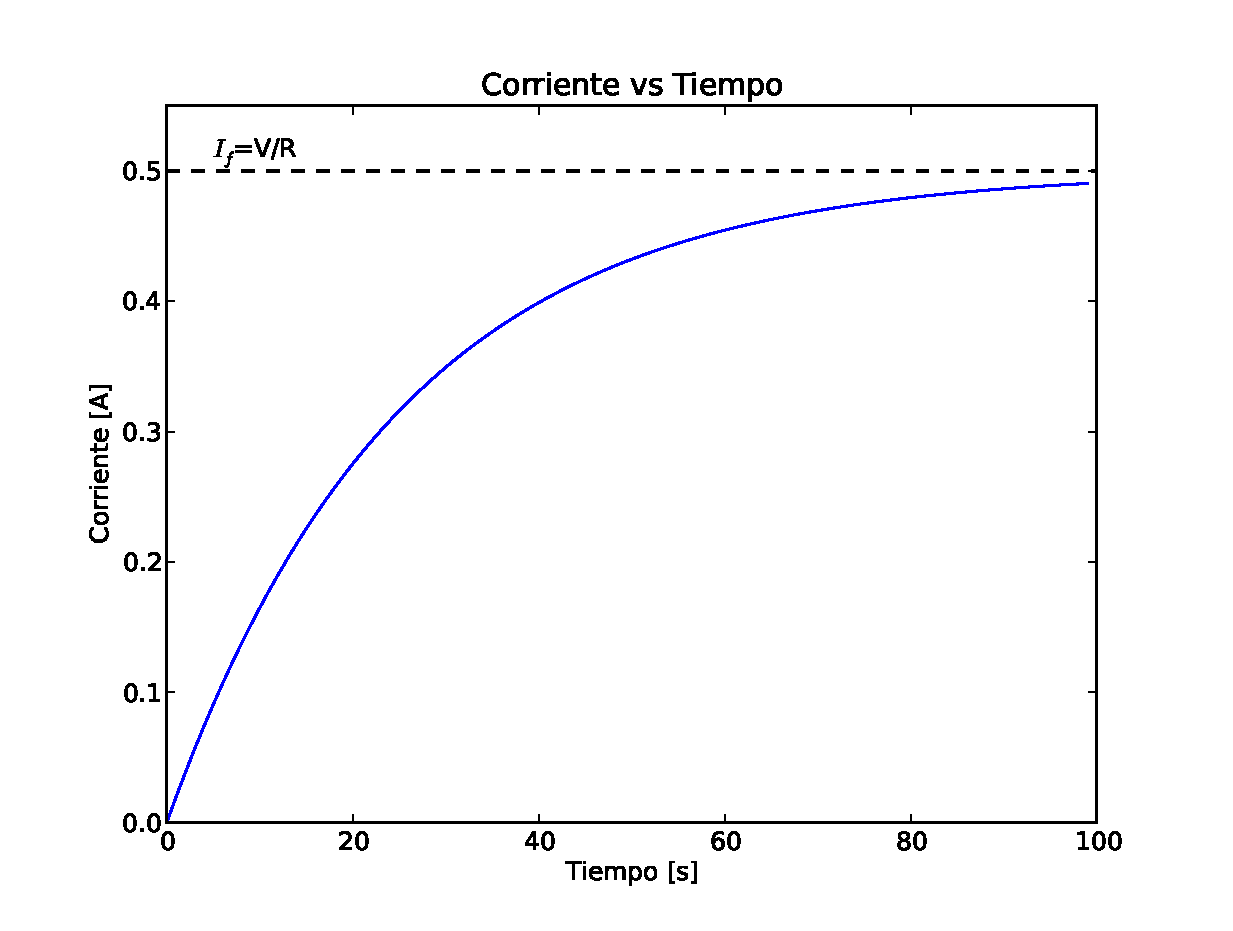
\includegraphics[scale=0.4]{RK2circuito.eps} 
% \end{figure}
% \end{frame}
% \begin{frame}[fragile]
% \fontsize{10}{10}\selectfont
% \begin{lstlisting}
% from numpy import *
% import matplotlib.pyplot as plt

% L=50.0
% R=20.0
% V=10.0
% h=0.1
% corriente=0
% I=[]
% I.append(0)

% for i in range(99):
%     k1=h*((-R/L)*corriente+(V/L))
%     k2=h*((-R/L)*(corriente+k1)+(V/L))
%     corriente=corriente+(k1+k2)*0.5
%     I.append(corriente)
% \end{lstlisting}
% \end{frame}
% \begin{frame}
% La rutina para la gráfica con \texttt{matplotlib} la pueden implementar sin mayor problema.
% \\
% \bigskip
% Nótese que el valor de corriente límite corresponde a $I_{f}=V/R$ que alcanzaría en un tiempo mucho mayor.
% \end{frame}
\end{document}